%!TEX root = skripsi.tex
%-----------------------------------------------------------------------------%
\chapter{\babLima}
%-----------------------------------------------------------------------------%
Bab ini menjelaskan mengenai hasil yang didapatkan dari eksperimen, serta evaluasi dan analisis terkait hasil tersebut.

%-----------------------------------------------------------------------------%
\section{Korpus Identik}
%-----------------------------------------------------------------------------%
Korpus identik berisi pasangan-pasangan kalimat Indonesia-Inggris sebanyak 88.919 kalimat untuk masing-masing bahasa.
%-----------------------------------------------------------------------------%

%-----------------------------------------------------------------------------%
\section{Pembuatan \textit{Sense Tagged Corpus} Bahasa Inggris}
Tabel \ref{table:sense-tagged-corpus} menunjukan jumlah token (kata) pada korpus bahasa Inggris dan yang diberikan \textit{tag sense} oleh IMS

\begin{table}
	\centering
	\caption{Jumlah \textit{instance} korpus bahasa Inggris}
	\label{table:sense-tagged-corpus}
	\begin{tabular}{|p{0.7cm}|p{4cm}|p{4cm}|}
		\hline
		No & Tipe & Jumlah
		\\ \hline
		1    & 
		Token (kata)   & 
		1.801.484
		\\ \hline
		2    & 
		Kata yang diberikan \textit{tag} oleh IMS     & 
		1.024.797 
		\\ \hline
	\end{tabular}
\end{table}

Berdasarkan proses pembuatan dan hasil dari \textit{sense tagged corpus} tersebut, dapat dilihat bahwa tidak semua kata diberikan \textit{sense} oleh IMS. Kata-kata sapaan seperti "I", "you", dan kata \textit{articles} yaitu "a", "the", "an". Selain itu, kata yang tidak terdapat pada model juga tidak diberi \textit{tag} (dilewati) oleh IMS. Tingkat kebenaran dari \textit{sense tag} yang diberikan bergantung dari model yang digunakan pada penelitian. Terdapat banyak kasus-kasus dimana pemberian \textit{sense} yang dilakukan adalah benar seperti misalnya pada kata "\textit{visitor}" yang diberikan \textit{tag} dengan \textit{sense key} 1:18:00::, yang mana berdasarkan wordnet Princeton "visitor\%1:18:00::" memiliki arti sebagai "\textit{someone who visits}". Contoh lain dari kata yang diberikan \textit{tag} dengan benar adalah "\textit{company}" pada konteks potongan kalimat "\textit{Plantation company PT ...}". Kata "\textit{company}" tersebut diberikan tag "company\%1:14:01::" yang berdasarkan wordnet Princeton memiliki makna "\textit{an institution created to conduct business}". Namun demikian, terjadinya kesalahan pemberian \textit{tag} pada kata terjadi pada kasus-kasus seperti: 

\begin{enumerate}
	\item Sebuah entitas diberikan \textit{tag} dimana entitas tersebut dianggap kata biasa. Contohnya adalah kata "Scotland Yard" dimana "Yard" pada kata tersebut diberikan \textit{tag} yang diartikan sebagai "\textit{a unit of length equal to 3 feet}". Hal ini menunjukan bahwa \textit{tool} belum dapat membedakan antara entitas yang memang tidak perlu diberikan \textit{tag} dan kata biasa (walaupun kata tersebut sudah memiliki huruf kapital).
	\item Kesalahan \textit{tag} dikarenakan \textit{training data} yang digunakan oleh model. Pada potongan kalimat "\textit{... FASB rule will cover such financial instruments as interest rate swaps financial ...}, kata "\textit{interest}" diberikan tag dengan makan "a sense of concern with and curiosity about someone or something". Berdasarkan konteks kalimat tersebut, dapat diketahui bahwa makna yang seharusnya didapat untuk kata "\textit{interest}" diatas ialah "bunga bank". Hal ini sepertinya terjadi karena data yang digunakan untuk \textit{training} model IMS memiliki ketidakseimbangan data untuk model kata "\textit{interest}" sehingga \textit{tag} yang diberikan lebih cenderung kepada "ketertarikan".
	\item Pemberian \textit{tag} pada \textit{multi word} token seperti "\textit{make up}" masih diberikan pada setiap kata. Berdasarkan percobaan untuk \textit{tagging} pada kata tersebut, kata "\textit{make}" dan "\textit{up}" masing-masing diberikan tag yang berbeda. Hal ini terjadi karena IMS mengolah kata demi kata dengan proses tokenisasi \textit{by default} menggunakan spasi. Setelah dilakukan pemeriksaan pada kata-kata yang terdapat pada model, kata \textit{make up} ternyata disimpan sebagai "make\_up". Berdasarkan pemeriksaan tersebut, diperlukan adanya \textit{pre-processing} terlebih dahulu untuk mengganti \textit{separator} kata multiword yang umumnya menggunakan spasi dengan "\_" agar IMS dapat memberikan \textit{tag multi word} tersebut dengan benar.
\end{enumerate}
%-----------------------------------------------------------------------------%

%-----------------------------------------------------------------------------%
\section{\textit{Word Alignment}}

%-----------------------------------------------------------------------------%

\subsection{}


\subsection{Evaluasi}
Evaluasi terhadap \textit{word alignment} dilakukan dengan membandingkan hasil Giza dengan anotasi manual yang dilakukan oleh dua anotator dengan indikator kualitatif berupa \textit{precision} dan \textit{recall}. 

\section{Pengumpulan Data}
%-----------------------------------------------------------------------------%
Tabel \ref{table:dataXML} menunjukkan spesifikasi dari dua jenis data XML Wikipedia digunakan untuk eksperimen yang diunduh dari situs Wikimedia.

\begin{table}
	\centering
	\caption{Dua jenis data XML Wikipedia}
	\label{table:dataXML}
		\begin{tabular}{|p{0.7cm}|p{4cm}|p{4cm}|p{2cm}|p{1.5cm}|}
			\hline
			No & Berkas & Jenis & Tangga Diambil & Ukuran \\ 
			\hline
			1    & 
			idwiki-20160901-pages-articles-multistream.xml.bz2   & \textit{Articles, templates, media/file descriptions}, dan \textit{primary meta-pages}  & 2016-09-02 13:24:24  & 
			381.3 MB  \\ \hline
			2    & 
			idwiki-20160901-pages-meta-history.xml.bz2     & 
			All pages with complete page edit history  & 
			2016-09-07 18:22:58  & 
			2.8 GB    \\ \hline
		\end{tabular}
\end{table}
\noindent Berkas pertama adalah XML semua artikel Wikipedia tanpa revisi, berkas kedua adalah Wikipedia \textit{revision history}. Kedua berkas merupakan data Wikipedia terakhir pada tanggal 1 September 2016. Jika dilihat ukuran, XML Wikipedia sudah sangat mencukupi kebutuhan data untuk penelitian ini.

%-------%
\section{Hasil Pengolahan Data}
%-----------------------------------------------------------------------------%
Ada dua jenis pengolahan data yang dilakukan, yang pertama adalah mengolah data Wikipedia semua artikel menjadi model \textit{word embedding} dan yang kedua adalah pengolahan data utama, yaitu mengubah data Wikipedia \textit{revision history} menjadi pasangan kandidat T dan H. Berikut adalah hasil yang diperoleh pada setiap tahap pengolahan data.
\begin{itemize}
	\item \textbf{Ekstraksi Teks }\\
	Ekstraksi teks dilakukan pada kedua berkas yang diunduh. Pada berkas pertama yang berukuran 381.3 MB, seluruh artikel dapat diekstraksi. Total artikel yang didapatkan adalah 386.357 artikel. Sedangkan, pada berkas kedua, tidak seluruh artikel yang diekstraksi karena keterbatasan-keterbatasan dalam penelitian ini. Total artikel hasil ekstraksi berkas kedua berjumlah 10.758 artikel yang berisikan 595.136 \textit{revision history}. Contoh keluaran dari proses ekstraksi XML semua artikel Wikipedia dapat dilihat pada gambar \ref{fig:hasil-ekstraksi}; sedangkan, XML Wikipedia Revision History pada gambar \ref{fig:revisi_induk}.
	
	\item \textbf{Pemenggalan Kalimat} \\
	Dari 386.357 artikel, total kalimat setelah dilakukan pemenggalan adalah 3.867.831 kalimat. Semua kalimat yang terdiri lebih dari dua kata akan digunakan untuk membentuk model \textit{word embedding}. 

	\item \textbf{Pemodelan Word Embedding} \\
	Model \textit{word embedding} dibentuk menggunakan data 3.867.831 kalimat bersih dan menghasilkan 3 buah berkas model (lihat pada tabel \ref{table:modelWE}).
	\begin{table}
		\centering
		\caption{Berkas model \textit{word embedding}}
		\label{table:modelWE}
		\begin{tabular}{|p{4cm}|p{2cm}|p{2.5cm}|}
			\hline
			Nama Berkas & Jenis & Ukuran \\ 
			\hline 
			word2vec   &  File  & 40.987 KB \\ \hline 
			word2vec.syn0.npy     & NPY File
			  & 
			227.472 KB \\ \hline
			word2vec.syn1neg.npy     & NPY File  & 
			227.472 KB \\ \hline
		\end{tabular}
	\end{table}
	
	\item\textbf{Pembentukan T dan H} \\
	Sebelum membentuk T dan H, teks induk dan revisi dipasangkan terlebih dahulu. Jumlah pasangan yang terbentuk adalah 584.377 pasang. Setelah melalui tahap pemrosesan, dihasilkan sejumlah 67.096 pasang T dan H. Pasangan T dan H yang terbentuk menunjukkan jenis \textit{entailment} yang terjadi adalah tingkat leksikal karena data didominasi dengan pasangan kalimat yang \textit{lexical overlap}-nya tinggi, yaitu pasangan yang memiliki banyak kesamaan kata. 
	
	\item \textbf{Anotasi Data Manual} \\
	Dari 500 data \textit{random} yang digunakan saat pelabelan manual, hanya 400 data saja yang akan digunakan sebagai bibit Co-training.  Penjelasan lebih lanjut dapat dilihat pada bagian \ref{sec:anotasi-manual}.
	
	\item \textbf{Ekstraksi fitur} \\
	Kombinasi fitur sepasang T dan H adalah fitur \textit{word embedding} serta fitur tambahan pada masing-masing kalimat T dan H (selanjutnya dibahas pada bagian \ref{sec:uji-rnn}). Sedangkan fitur untuk komentar penulis adalah kemunculan N-gram tertentu (selanjutnya dibahas di bagian \ref{sec:uji-fitur2}). Hanya 15.000 dari 67.096 pasang T dan H serta komentar penulis yg dapat diubah menjadi vektor fitur tersebut karena keterbatasan waktu dan penyimpanan. 
\end{itemize}

%-------%
\section{Hasil Anotasi Manual} \label{sec:anotasi-manual}
%-----------------------------------------------------------------------------%
Sebelum melakukan anotasi, para anotator akan diuji pemahamannya terlebih dahulu. Anotator yang cukup paham mengenai permasalahan \textit{Textual Entailment}, yaitu ketika tingkat persetujuan anotasi \saya~ dan anotator tersebut melebihi 0,5 berdasarkan perhitungan Cohen's Kappa, akan lanjut ke tahap anotasi data yang sebenarnya. Sebelum uji coba, seluruh anotator diberi panduan anotasi untuk meningkatkan pemahaman mereka terhadap \textit{Textual Entailment}. Ukuran data uji coba adalah 15 data yang dipilih secara khusus agar dapat mencakup berbagai kasus. Berikut adalah tabel hasil anotasi uji coba.

\begin{table}
	\centering
	\caption{Kappa antara \saya~dan masing-masing anotator pada data ujicoba}
	\label{table:cohensKappa}
	\begin{tabular}{lllllll}
		\hline
		\multicolumn{1}{|l|}{anotator ke-} & \multicolumn{1}{l|}{1} & \multicolumn{1}{l|}{2} & \multicolumn{1}{l|}{3} & \multicolumn{1}{l|}{4} & \multicolumn{1}{l|}{5} & \multicolumn{1}{l|}{6} \\ \hline
		\multicolumn{1}{|l|}{\textit{agreement}} & \multicolumn{1}{l|}{0.867} & \multicolumn{1}{l|}{0.8} & \multicolumn{1}{l|}{0.667} & \multicolumn{1}{l|}{0.8} & \multicolumn{1}{l|}{1} & \multicolumn{1}{l|}{0.8} \\ \hline
		\multicolumn{1}{|l|}{Kappa} & \multicolumn{1}{l|}{0.865} & \multicolumn{1}{l|}{0.798} & \multicolumn{1}{l|}{0.663} & \multicolumn{1}{l|}{0.798} & \multicolumn{1}{l|}{1} & \multicolumn{1}{l|}{0.798} \\ \hline
		\multicolumn{7}{l}{} \\ \hline
		\multicolumn{1}{|l|}{anotator ke-} & \multicolumn{1}{l|}{7} & \multicolumn{1}{l|}{8} & \multicolumn{1}{l|}{9} & \multicolumn{1}{l|}{10} & \multicolumn{1}{l|}{11} & \multicolumn{1}{l|}{12} \\ \hline
		\multicolumn{1}{|l|}{\textit{agreement}} & \multicolumn{1}{l|}{0.933} & \multicolumn{1}{l|}{0.867} & \multicolumn{1}{l|}{0.8} & \multicolumn{1}{l|}{0.933} & \multicolumn{1}{l|}{0.933} & \multicolumn{1}{l|}{0.867} \\ \hline
		\multicolumn{1}{|l|}{Kappa} & \multicolumn{1}{l|}{0.932} & \multicolumn{1}{l|}{0.865} & \multicolumn{1}{l|}{0.798} & \multicolumn{1}{l|}{0.932} & \multicolumn{1}{l|}{0.932} & \multicolumn{1}{l|}{0.865} \\ \hline
	\end{tabular}
\end{table}
\noindent Dari tabel \ref{table:cohensKappa}, terlihat bahwa nilai Kappa semua anotator melampaui batas yang ditentukan, sehingga semua anotator dapat melanjutkan ke tahap berikutnya.

Selain menghitung persetujuan antara \saya~dan anotator, persetujuan secara keseluruhan perlu dihitung. Persetujuan keseluruhan pada data uji coba akan menjadi \textit{baseline} untuk nilai persetujuan keseluruhan pada data yang sebenarnya. Apabila nilai persetujuan keseluruhan pada data yang sebenarnya lebih baik dari persetujuan keseluruhan di data uji coba, data uji coba benar tergolong representatif.
\begin{table}
	\centering
	\caption{Hasil anotasi uji coba}
	\label{table:data-fleiss}
	\begin{tabular}{|p{2cm}|c|c|c|}
		\hline
		\textbf{} & \textbf{Label E} & \textbf{Label C} & \textbf{Label U} \\ \hline
		\textbf{Data-1} & 13 & 0 & 0 \\ \hline
		\textbf{Data-2} & 13 & 0 & 0 \\ \hline
		\textbf{Data-3} & 1 & 2 & 10 \\ \hline
		\textbf{Data-4} & 9 & 4 & 0 \\ \hline
		\textbf{Data-5} & 13 & 0 & 0 \\ \hline
		\textbf{Data-6} & 10 & 1 & 2 \\ \hline
		\textbf{Data-7} & 8 & 1 & 4 \\ \hline
		\textbf{Data-8} & 3 & 1 & 9 \\ \hline
		\textbf{Data-9} & 12 & 0 & 1 \\ \hline
		\textbf{Data-10} & 4 & 0 & 9 \\ \hline
		\textbf{Data-11} & 13 & 0 & 0 \\ \hline
		\textbf{Data-12} & 13 & 0 & 0 \\ \hline
		\textbf{Data-13} & 11 & 2 & 0 \\ \hline
		\textbf{Data-14} & 13 & 0 & 0 \\ \hline
		\textbf{Data-15} & 13 & 0 & 0 \\ \hline
	\end{tabular}
\end{table}	
\noindent Isi tabel menunjukkan jumlah anotator yang sepakat melabeli data pada baris tertentu dengan label pada kolom tertentu. Nilai Kappa yang dihasilkan berdasarkan tabel di atas adalah 0.432 dengan \textit{overall agreement} 0.783. Jika merujuk pada pengukuran \textit{agreement} di gambar \ref{table:skalaKappa}, nilai tersebut menunjukkan bahwa tingkat persetujuan antar anotator tergolong menengah.  

Setelah anotasi, masing-masing datum memiliki 3 label (dapat seragam maupun berbeda-beda), yaitu dari penilaian anotator 1, 2, dan 3. Tingkat persetujuan anotasi dari tiga anotator tersebut kemudian dihitung, \textit{overall agreement} yang dihasilkan sebesar 0.86 dan Kappa sebesar 0.729. Nilai tersebut menunjukkan bahwa pada data yang sebenarnya persetujuan lebih tinggi dibandingkan data uji. Bisa disimpulkan bahwa, data uji yang berukuran kecil tersebut merupakan sampel data yang representatif dan mengandung kasus-kasus yang ambiguitasnya tinggi.

Sebuah datum seharusnya hanya memiliki satu label saja, yaitu E, U, atau C. Oleh karena itu, label pada setiap datum perlu ditentukan dengan cara memilih label dengan keputusan terbanyak. Apabila label E, C, dan U muncul bersama pada satu datum, langkah yang dilakukan adalah menganalisis lebih dalam datum tersebut dan memutuskan label mana yang lebih tepat, umumnya label akan mengarah ke U. Kemudian, data yang sudah memiliki label tersebut akan kami analisis dari segi jumlahnya. Tujuannya adalah untuk mengetahui beberapa hal diantaranya pola pada pasangan T dan H. Setelah dianalisis kami mendapatkan hasil seperti pada tabel \ref{table:dataEUC}.
\begin{table}
	\centering
	\caption{Jumlah data per label hasil notasi}
	\label{table:dataEUC}
	\begin{tabular}{|c|c|c|c|}
		\hline
		\textbf & Label E & Label U & label C \\ \hline
		Jumlah  & 323 & 54 & 123 \\ \hline
	\end{tabular}
\end{table}
Perbandingan jumlah label pada tabel \ref{table:dataEUC} tidak seimbang dan dikhawatirkan dapat  mempengaruhi hasil klasifikasi menjadi lebih dominan ke suatu label. Untuk mencegah hal tersebut terjadi, dilakukan langkah-langkah berikut. 
\begin{itemize}
	\item Menggabungkan label C dan U menjadi label baru, yaitu NE yang berarti \textit{not entail}. Langkah ini diambil dengan pertimbangan bahwa data C dan U masih terlalu sedikit. Setelah label digabungkan, hasil data Textual Entailment pada penelitian ini akan \textit{binary}, yaitu E dan NE.
	\item Memangkas jumlah data berlabel E dari 323 menjadi 223, agar jumlah data berlabel E tidak dominan.
\end{itemize}
\noindent Setelah melakukan langkah-langkah tersebut, bibit yang diperoleh berkurang menjadi 400 data dengan perbandingan label E dan NE adalah 223:177.

%-----------------------------------------------------------------------------%
\section{Pengujian Arsitektur RNN} \label{sec:uji-rnn}
%-----------------------------------------------------------------------------%
Sebelum melakukan Co-training, terlebih dahulu dilakukan pemilihan arsitektur pada \textit{view} pertama. Kedua arsitektur tersebut diuji menggunakan metode 10-fold \textit{cross validation}  dengan terhadap data hasil proses anotasi manual atau calon bibit Co-training. Hasil \textit{cross validation} terdapat di tabel \ref{table:arsitekturRNN}. 
\begin{table}
	\centering
	\caption{Hasil \textit{cross validation} dua arsitektur RNN}
	\label{table:arsitekturRNN}
	\begin{tabular}{|c|c|}
		\hline
		Arsitektur RNN tanpa fitur tambahan & 0.58 \\ \hline
		Arsitektur RNN dengan fitur tambahan & 0.69 \\ \hline
	\end{tabular}
\end{table}
\textit{Cross validation} menggunakan program dalam bahasa Python yang dibuat dengan menambahkan \textit{library} Keras\footnote{https://keras.io/}. \textit{Library} Keras menyediakan berbagai \textit{neural network classifier}, seperti LSTM dan \textit{feed forward neural network}. Pada kedua percobaan, tahap \textit{train} data pada masing-masing RNN menggunakan jumlah \textit{epoch} yang sama, yaitu 200 \textit{epoch}. Jumlah \textit{epoch} dipilih secara heuristik dengan pertimbangan jumlah tersebut tidak terlalu kecil dan juga tidak terlalu besar. Penentuan jumlah \textit{epoch} seharusnya dilakukan dengan beberapa kali percobaan, namun dikarenakan waktu yang tidak mencukupi, \textit{epoch} langsung ditentukan sebesar 200.


%-----------------------------------------------------------------------------%
\section{Pemilihan Fitur View Kedua} \label{sec:uji-fitur2}
%-----------------------------------------------------------------------------%
Program Weka GUI digunakan untuk menentukan fitur pada \textit{view} kedua. Fitur untuk \textit{view} kedua berupa jumlah kemunculan unigram, bigram, dan trigram terbanyak pada komentar penulis dari seluruh data. Oleh karena itu, sebelum mendaftarkan apa saja fitur view kedua, frekuensi kemunculan N-gram pada data terlebih dahulu harus dibuat. 
Dari 67.000 pasang T dan H serta komentar penulis yang dihasilkan, dihitung kemunculan dari setiap unigram, bigram, dan trigram yang terdapat pada teks komentar. Kemudian kemunculan tersebut diurutkan berdasarkan jumlah terbanyak. N-gram yang dengan frekuensi yang banyak tersebut tidak langsung digunakan sebagai fitur, N-gram tersebut harus terlebih dahulu dianalisis dan dipilih, mana yang merupakan N-gram yang dapat merepresentasikan isi komentar. Pemilihan dilakukan manual dan menggunakan heuristik. Total ada sebanyak 74 buah N-gram yang digunakan sebagai rancangan fitur awal. Tabel \ref{table:n-gram} menunjukkan contoh dari N-gram tersebut.
\begin{table}
	\centering
	\caption{Contoh N-gram yang kemunculannya digunakan sebagai fitur}
	\label{table:n-gram}
	\begin{tabular}{|p{3cm}|p{9cm}|}
		\hline
		Unigram & sunting, revisi, kembali, ubah, ganti, menolak, tolak, mengembalikan, batal, rapikan, perbaikan, copyedit, replaced \\ \hline
		Bigram & ke versi, versi terakhir, suntingan special, dikembalikan ke, penggantian teks, teks otomatis, bicara dikembalikan, mengembalikan revisi \\ \hline		
		Trigram & teks terakhir oleh, perubahan terakhir oleh, menolak perubahan teks, menggunakan mesin wikipedia, dengan menggunakan mesin, replaced beliau dia, pada masa di, di tahun pada, di masa pada, masa pada masa \\ \hline
	\end{tabular}
\end{table}
Fitur jumlah kemunculan semua N-gram yang dipilih belum tentu akan menjadi kombinasi fitur yang paling baik. Oleh karena itu, digunakan fitur  \textit{select attribute} pada Weka GUI dengan metode \textit{genetic search} untuk memilih kombinasi fitur terbaik. Kombinasi ini didapat berdasarkan hasil training 500 data yang sebelumnya sudah dilabeli secara manual. Setelah melalui proses \textit{select attribute}, jumlah fitur tereduksi menjadi hanya 22 buah fitur jumlah kemunculan N-gram. 


%-----------------------------------------------------------------------------%
\section{Pengujian Classifier View Kedua}
%-----------------------------------------------------------------------------%
Kombinasi fitur terbaik hasil dari tahap pemilihan fitur menggunakan \textit{select attribute} pada Weka digunakan sebagai fitur untuk percobaan \textit{k-fold} \textit{cross validation}. \textit{Cross validation} dengan \textit{k=10} tersebut diujikan kepada beberapa \textit{classifier}. \textit{Classifier} untuk \textit{view} kedua belum ditentukan sebelumnya, namun ada beberapa \textit{classifier} yang sudah direncanakan akan dicoba. Semua \textit{classifier} yang akan digunakan tersedia di Weka GUI. Sama seperti saat tahap pemilihan atribut, \textit{cross validation} dilakukan terhadap data hasil anotasi manual. Berikut adalah hasil dari \textit{cross validation}.
\begin{table}
	\centering
	\caption{Hasil \textit{cross validation} beberapa \textit{classifier} di Weka}
	\label{table:classifierWeka}
	\begin{tabular}{|c|c|}
		\hline
		Classifier & Akurasi \\ \hline
		Decision Tree (J48) & 0.61 \\ \hline		
		Multilayer Perceptron & 0.626 \\ \hline
		Bayesian Network & 0.61 \\ \hline
		Naive Bayes & 0.626 \\ \hline
		Multinomial Naive Bayes & 0.636 \\ \hline
	\end{tabular}
\end{table}
\noindent Walaupun nilai akurasi tidak terlihat jauh berbeda, \textit{classifier} Multinomial Naive Bayes memberikan hasil yang baik di antara beberapa percobaan lain, dengan akurasi 0.636. Multinomial Naive Bayes digunakan sebagai \textit{classifier} pada \textit{view} kedua Co-training.
%-----------------------------------------------------------------------------%
\section{Co-training}
%-----------------------------------------------------------------------------%
Co-training hanya dilakukan terhadap 15.000 dari 67.096 data yang dimiliki karena keterbatasan pada penelitian ini, diantaranya waktu dan kapasitas penyimpanan untuk melakukan komputasi data. Bibit yang digunakan sejumlah 400 data.

Data hasil klasifikasi hanya diambil yang terbaik untuk ditambahkan pada data berlabel. Untuk mengurangi kemungkinan bertambahnya data yang tidak akurat pada \textit{training data}, ada batasan yang harus dipenuhi oleh masing-masing data yang akan ditambahkan, yaitu data diklasifikasikan ke dalam label yang sama oleh kedua \textit{classifier} pada Co-training dengan tingkat kepercayaan di atas 0.9 untuk \textit{classifier} \textit{view} pertama dan di atas 0.5 untuk \textit{view} kedua. Angka tersebut dipilih berdasarkan anggapan bahwa \textit{view} pertama akan lebih informatif dibandingkan dengan \textit{view} kedua. Sehingga, nilai kepercayaan RNN dalam melabeli data disyaratkan sangat tinggi.

Setelah sejumlah data terbaik terpilih sebagai calon data tambahan, jumlah label dari data tersebut harus dibandingkan. Apabila jumlah label E:NE berada melebihi 5:4 atau kurang dari 4:5, data yang jumlahnya berlebih harus dipangkas hingga perbandingan E:NE menjadi 1:1. Batasan ini harus ditentukan agar ke depannya tidak terjadi ketimpangan jumlah label pada data. Batasan tersebut diambil berdasarkan perbandingan data berlabel mula-mula yaitu 223:177 yang mendekati dengan perbandingan 5:4.

Pada bagian \ref{sec:cotrain}, disebutkan bahwa \textit{stopping condition} dari Co-training pada penelitian ini adalah ketika kedua \textit{classifier} tidak mampu menyepakati satu pun label yang sama dalam \textit{n} iterasi berurutan. Selain itu, algoritme Co-training pada gambar \ref{fig:Co-training} menunjukkan ada \textit{k} buah data yang diambil dari data tidak berlabel setiap iterasi. Nilai \textit{n} dan \textit{k} berturut-turut ditentukan sebesar 3 dan 500. Nilai tersebut ditentukan setelah percobaan kombinasi \textit{n} dan \textit{k} pada Co-training dilakukan.
\begin{itemize}
	\item Percobaan 1 dengan \textit{n}=3 dan \textit{k}=100\\ Percobaan 1 terhenti pada iterasi 13, dimana pada iterasi 10, 11, dan 12, data terbaik yang dihasilkan berjumlah 0. 
	\item Percobaan 2 dengan \textit{n}=5 dan \textit{k}=100\\ Percobaan 2 terhenti pada iterasi 15. Sama seperti percobaan 1, iterasi 10, 11, 12, 13, dan 14 tidak menghasilkan data terbaik satu pun. 
	\item Percobaan 3 dengan \textit{n}=3 dan \textit{k}=500\\ Percobaan 3 masih berjalan hingga iterasi ke 93. Jumlah data terbaik yang dihasilkan pun cukup menjanjikan. Percobaan ini yang kemudian digunakan hingga akhir penelitian ini.
\end{itemize}
Jika jumlah data tidak berlabel yang digunakan dalam sebuah iterasi terlalu kecil, iterasi akan cepat berhenti karena kemungkinan tidak adanya data terbaik yang diperoleh pada tiap iterasi menjadi lebih besar.

\subsection{Hasil Co-training}
Hasil tiap iterasi dari percobaan Co-training disimpan untuk dievaluasi dan dianalisis. Hasil yang dikeluarkan berupa pasangan T dan H serta komentar penulis yang sudah diberi label. Gambar \ref{fig:hasil-cotrain} menunjukkan contoh hasil dari Co-training pada salah satu iterasi.
\begin{figure}
	\centering
	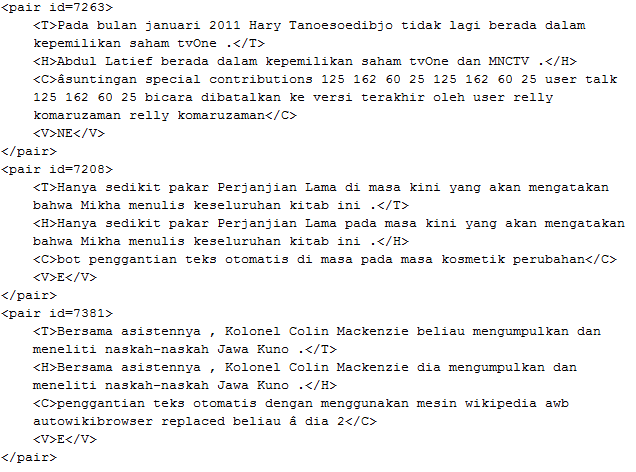
\includegraphics[width=1\linewidth]{pics/hasil-cotrain}
	\caption{Contoh hasil Co-training pada salah satu iterasi}
	\label{fig:hasil-cotrain}
\end{figure}

Setelah program Co-training terhenti, terdapat 1.857 data yang berhasil dilabeli dari total 15.000 data tidak berlabel yang digunakan, dengan perbandingan jumlah data label E:NE adalah 927:930. Pola jumlah data pada setiap iterasi dapat dilihat pada gambar \ref{pic:jumlah-iterasi}.
\begin{figure}
	\centering
	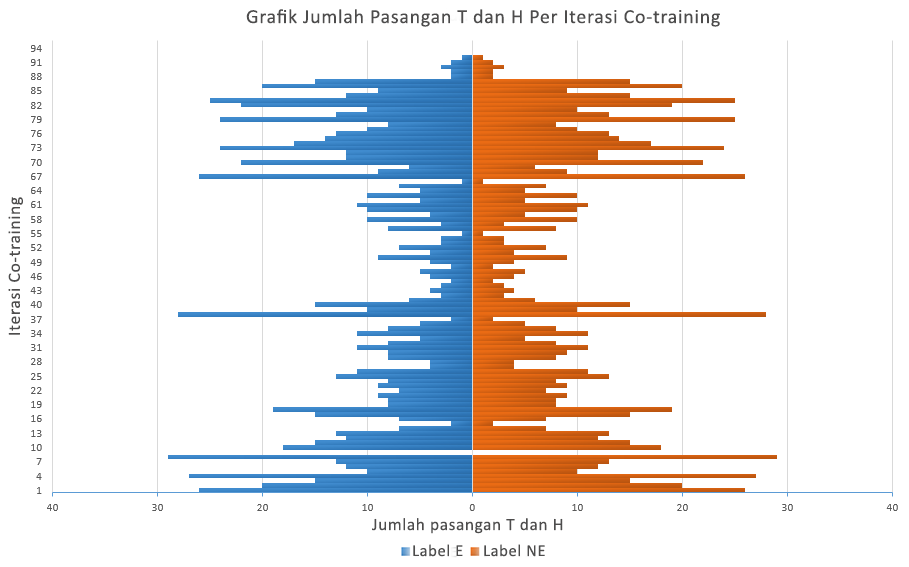
\includegraphics[width=1\linewidth]{pics/grafik-jumlah}
	\caption{Jumlah data yang diperoleh pada tiap iterasi}
	\label{pic:jumlah-iterasi}
\end{figure}	
\noindent Jumlah data yang diperoleh di tiap iterasi sangat acak dan beragam, mulai dari yang sangat kecil hingga sangat besar, bahkan pada iterasi ke-9, Co-training tidak mengeluarkan data berlabel  satu pun. Jumlah data tersebut berada di rentang 0 hingga 58. Dengan mempertimbangkan pola yang acak dan beragam, evaluasi dilakukan tidak per iterasi, melainkan per 5 iterasi. Bila dilihat dari segi perbandingan jumlah label E dan NE, Co-training yang dirancang dapat mengatasi masalah ketidakseimbangan yang dikhawatirkan di awal. Kemungkinan besar data yang diperoleh dipangkas jumlahnya karena terlihat dari hasil perbandingan label pada tiap iterasi yang hampir semuanya 1:1. Hasil perbandingan antara E dan NE yang hampir sama tersebut menjadi salah satu kekurangan pada penelitian ini. Seharusnya pemangkasan tidak berdasarkan perbandingan jumlah data hasil pelabelan, namun berdasarkan perbandingan jumlah data berlabel keseluruhan.

\subsection{Evaluasi Co-training}
Evaluasi dilakukan setiap 5 iterasi sekali (untuk selanjutnya disebut kelompok iterasi) dengan cara mengambil sampel acak sebanyak 13 data berlabel E dan 13 data berlabel NE dari total data dalam sebuah kelompok iterasi. Data yang terpilih akan dievaluasi secara manual.  Tabel \ref{table:akurasi-iterasi} menunjukkan akurasi setiap kelompok iterasi setelah evaluasi.
\begin{table}
	\centering
	\caption{Jumlah data pada setiap iterasi}
	\label{table:akurasi-iterasi}
	\begin{tabular}{|p{0.6cm}|p{0.9cm}|p{0.9cm}|p{1.1cm}|p{1.2cm}|p{1.2cm}|p{1.2cm}|p{1.2cm}|p{1.7cm}|}
		\hline
		No & Label E & Label NE & Jumlah & Sampel E Tepat & Sampel NE Tepat & Akurasi Label E & Akurasi Label NE & Rata-rata Akurasi \\ \hline
		1 & 98 & 98 & 196 & 11 & 9 & 0.85 & 0.69 & 0.77 \\ \hline
		2 & 72 & 72 & 144 & 12 & 11 & 0.92 & 0.85 & 0.88 \\ \hline
		3 & 49 & 49 & 98 & 13 & 9 & 1.00 & 0.69 & 0.85 \\ \hline
		4 & 57 & 57 & 114 & 13 & 10 & 1.00 & 0.77 & 0.88 \\ \hline
		5 & 46 & 46 & 92 & 13 & 12 & 1.00 & 0.92 & 0.96 \\ \hline
		6 & 35 & 36 & 71 & 13 & 11 & 1.00 & 0.85 & 0.92 \\ \hline
		7 & 43 & 43 & 86 & 13 & 10 & 1.00 & 0.77 & 0.88 \\ \hline
		8 & 60 & 60 & 120 & 11 & 6 & 0.85 & 0.46 & 0.65 \\ \hline
		9 & 18 & 18 & 36 & 11 & 8 & 0.85 & 0.62 & 0.73 \\ \hline
		10 & 24 & 24 & 48 & 12 & 12 & 0.92 & 0.92 & 0.92 \\ \hline
		11 & 18 & 18 & 36 & 13 & 5 & 1.00 & 0.38 & 0.69 \\ \hline
		12 & 35 & 36 & 71 & 12 & 9 & 0.92 & 0.69 & 0.81 \\ \hline
		13 & 38 & 38 & 76 & 13 & 4 & 1.00 & 0.31 & 0.65 \\ \hline
		14 & 64 & 64 & 128 & 12 & 3 & 0.92 & 0.23 & 0.58 \\ \hline
		15 & 79 & 79 & 158 & 6 & 11 & 0.46 & 0.85 & 0.65 \\ \hline
		16 & 68 & 69 & 137 & 6 & 10 & 0.46 & 0.77 & 0.62 \\ \hline
		17 & 78 & 78 & 156 & 8 & 10 & 0.62 & 0.77 & 0.69 \\ \hline
		18 & 42 & 42 & 84 & 5 & 10 & 0.38 & 0.77 & 0.58 \\ \hline
	\end{tabular}
\end{table}
\noindent Nilai akurasi total pada label E adalah 0.82, akurasi total label NE adalah 0.67, dan akurasi untuk data keseluruhan adalah 0.76. Jika hasil akurasi pada kelompok iterasi di-plot pada sebuah grafik (lihat grafik \ref{pic:akurasi-iterasi}), dapat disimpulkan bahwa akurasi Co-training cenderung mengalami penurunan. Hasil evaluasi juga menunjukkan kecenderungan pelabelan label E lebih akurat dibandingkan NE.
\begin{figure}
	\centering
	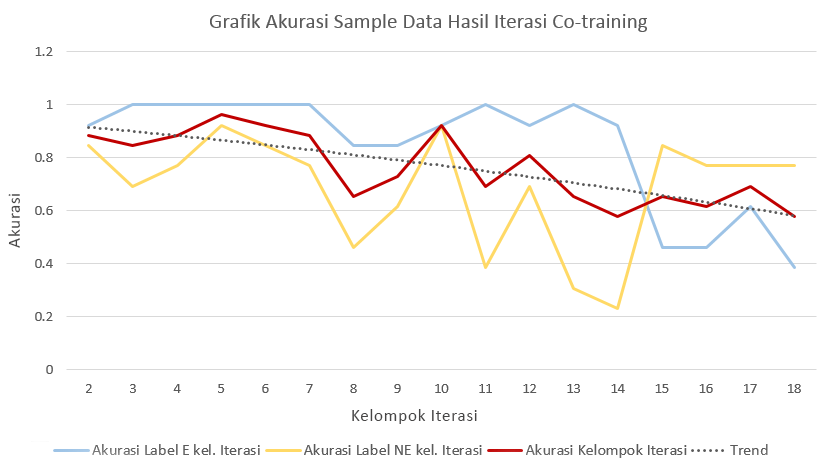
\includegraphics[width=1\linewidth]{pics/grafik-akurasi}
	\caption{Akurasi pada setiap kelompok iterasi}
	\label{pic:akurasi-iterasi}
\end{figure}
Evaluasi dengan data metode \textit{random sampling} ini sebaiknya dilakukan berkali-kali hingga nilai akurasi konvergen. Kemudian, nilai akurasi total dihitung dengan cara mencari nilai rata-rata dari seluruh akurasi \textit{sampling}. 

\subsection{Analisis Co-training}
Jumlah data pada korpus yang dihasilkan cukup besar apabila dibandingkan dengan jumlah bibit yang dimasukkan yaitu 400 data. Namun, jumlah hasil data tersebut masih terbilang kecil bila dibandingkan dengan ukuran data tidak berlabel semula, yaitu belum mencapai 13\% dari total data tidak belabel. Hal tersebut menunjukkan bahwa Co-training yang dibangun masih belum percaya diri untuk mampu melabeli data yang tersisa. 

Data yang diekstrak dengan Wikipedia cenderung didominasi oleh data \textit{textual entailment} tingkat leksikal dan data yang tingkat \textit{lexical overlap}-nya tinggi. Data \textit{textual entailment} tingkat leksikal yang diekstrak pun kemungkinan besar berlabel E. Sedangkan, label NE umumnya diberikan pada data yang teks antara T dan H nya jauh berbeda. Oleh karena itu, Co-training dapat lebih mudah mengidentifikasikan sebagian besar label data tersebut sehingga akurasi yang dihasilkan menjadi baik. 

Setelah melakukan evaluasi, ditemukan beberapa kekurangan dari Co-training yang diajukan, di antaranya:
\begin{enumerate}
	\item Co-training membuat kesalahan pelabelan akibat data penggunaan bahasa asing pada data.
	\begin{figure}
		\centering
		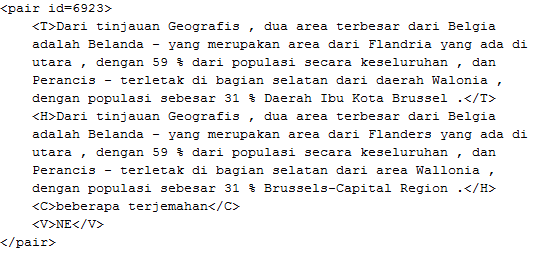
\includegraphics[width=0.85\linewidth]{pics/kasus-1-1}
		\caption{Contoh kesalahan pelabelan}
		\label{pic:kasus-1-1}
	\end{figure}
	\noindent Gambar di atas menunjukkan contoh data yang mengalami kesalahan pelabelan untuk suatu label yang seharusnya E. Penyebabnya adalah beberapa kata pada kalimat pada H menggunakan bahasa Inggris.
	\item Co-training memprediksi label E dikarenakan \textit{lexical overlap} antara T dan H cukup tinggi. Padahal perbedaan leksikal antara T dan H tersebut mengakibatkan perubahan makna pada teks.
	\begin{figure}
		\centering
		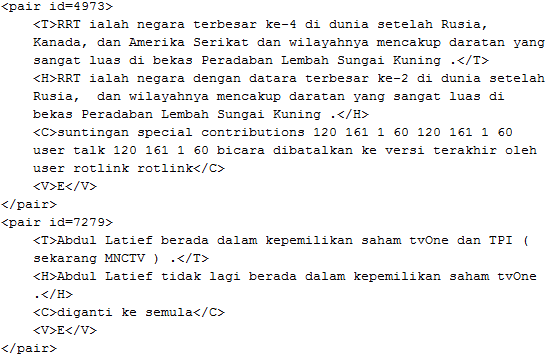
\includegraphics[width=0.85\linewidth]{pics/kasus-1-2}
		\caption{Contoh kesalahan pelabelan}
		\label{pic:kasus-1-2}
	\end{figure}
	\noindent Gambar di atas menunjukkan contoh kesalahan pelabelan untuk suatu data yang \textit{lexical overlap}-nya tinggi namun seharusnya berlabel NE. Co-training belum bisa mendeteksi perbedaan angka pada (data pertama) dan penggunaan kata negasi (pada data kedua).
	\item Co-training membuat kesalahan pelabelan pada data yang seharusnya mudah dideteksi nilai \textit{entailment}-nya, seperti data yang memiliki \textit{lexical overlap} tinggi dan seharusnya berlabel E.
	\begin{figure}
		\centering
		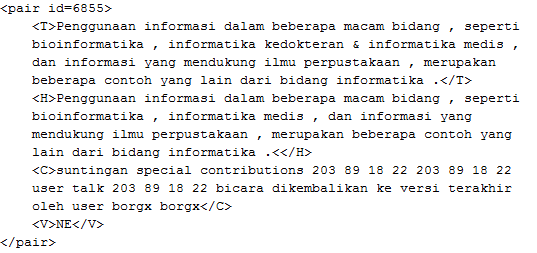
\includegraphics[width=0.85\linewidth]{pics/kasus-2}
		\caption{Contoh kesalahan pelabelan}
		\label{pic:kasus-2}
	\end{figure}
	\noindent Gambar \ref{pic:kasus-2} menunjukkan tingkat kesamaan antara T dan H yang tinggi, namun diberi penilaian NE oleh Co-training. Kesalahan seperti ini sulit untuk diprediksi penyebabnya.	
	\item Semakin lama Co-training dilakukan, data yang dihasilkan akan semakin jenuh. Pada kelompok iterasi-iterasi terakhir, data berlabel yang diperoleh semakin jenuh, yaitu memiliki jenis revisi yang serupa, misalnya hanya merevisi kata "dia" menjadi "beliau", "Cina" menjadi "Tiongkok", atau "di" menjadi "pada". Hal ini bisa disebabkan karena koleksi data berlabel yang tersisa sudah tidak bervariasi lagi.
\end{enumerate}

Selain memiliki kasus-kasus kesalahan, ada pula kasus ketika Co-training bisa memberikan label yang tepat pada kasus yang terbilang sulit diprediksi oleh komputer. Contohnya terdapat pada gambar berikut.
\begin{figure}
	\centering
	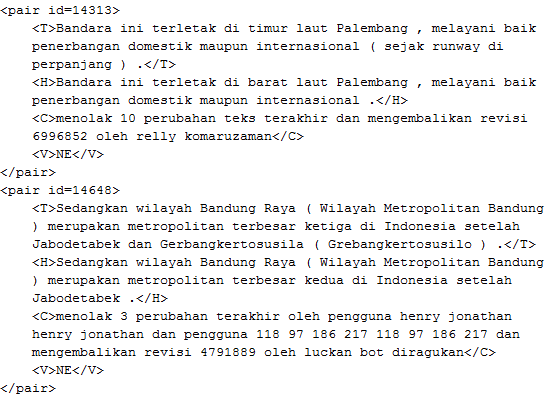
\includegraphics[width=0.85\linewidth]{pics/bagus-1}
	\caption{Contoh pelabelan berhasil}
	\label{pic:bagus-1}
\end{figure}
\noindent Contoh pada gambar di atas bertentangan dengan kasus yang ditemukan pada poin kedua pembahasan kekurangan Co-training. Pada gambar \ref{pic:bagus-1}, Co-training menunjukkan kehandalannya dalam memberikan label NE untuk data yang \textit{lexical overlap}-nya tinggi namun mengandung makna yang berbeda. Hal tersebut bisa disebabkan karena dukungan dari \textit{view} komentar.

Pola yang ditunjukkan oleh hasil dari proses Co-training tidak dapat diprediksi. Beberapa contoh kasus yang sama atau serupa, diberikan label yang berbeda oleh Co-training. Penyebabnya kemungkinan besar adalah karena setiap iterasi Co-training dilatih oleh data berlabel tambahan. Sehingga sulit untuk mengetahui pola pelabelan Co-training. Salah satu penyebab kekurangan Co-training ini adalah penggunaan data bibit yang \saya~akui masih terbilang kecil, apalagi untuk penelitian \textit{deep learning}. Namun, jika dilihat dari akurasi, Co-training cukup memberikan hasil yang baik.

